%!TEX TS-program = xelatex
%!TEX encoding = UTF-8 Unicode
%!BIB TS-program = bibtex
%!TeX spellcheck = en_US
\documentclass[12pt]{article}
\usepackage[english]{babel}
\usepackage{url}
\usepackage[utf8x]{inputenc}
\usepackage{amsmath}
\usepackage{graphicx}
\graphicspath{{images/}}
\usepackage{parskip}
\usepackage{fancyhdr}
\usepackage{vmargin}
\usepackage{enumerate}
\usepackage[T1]{fontenc}
\usepackage{newpxtext,newpxmath}
\usepackage{booktabs}
\usepackage{siunitx}
\usepackage[version=4]{mhchem}
\usepackage{hyperref}
\usepackage{bm}
\usepackage{breqn}
\usepackage{miller}
\usepackage{braket}
\usepackage[space]{grffile}   % include graphics with spaces in their path


\setmarginsrb{1 cm}{2.5 cm}{1 cm}{2.5 cm}{1 cm}{1.5 cm}{1 cm}{1.5 cm}
\sisetup{inter-unit-product = \ensuremath{{}\cdot{}}}
\DeclareTextCommand{\nobreakspace}{T1}{\leavevmode\nobreak\ }

\title{Solid State Physics HW 6}								% Title
\author{XYZ}								% Author
\date{}											% Date

\makeatletter
\let\thetitle\@title
\let\theauthor\@author
\let\thedate\@date
\makeatother

\pagestyle{fancy}
\fancyhf{}
\rhead{\theauthor}
\lhead{\thetitle}
\cfoot{\thepage}

\newcommand*{\rmn}[1]{\romannumeral#1}
\newcommand*{\RMN}[1]{\uppercase\expandafter{\romannumeral#1}}
 \newenvironment{mpmatrix}{\begin{medsize}\begin{pmatrix}}%
                {\end{pmatrix}\end{medsize}}%
\newcount\colveccount
\newcommand*\colvec[1]{
    \global\colveccount#1
    \begin{pmatrix}
        \colvecnext
    }
    \def\colvecnext#1{
        #1
        \global\advance\colveccount-1
        \ifnum\colveccount>0
        \\
        \expandafter\colvecnext
        \else
    \end{pmatrix}
    \fi
}
\newcommand*{\tran}{^{\mkern-1.5mu\mathsf{T}}}

\begin{document}

%%%%%%%%%%%%%%%%%%%%%%%%%%%%%%%%%%%%%%%%%%%%%%%%%%%%%%%%%%%%%%%%%%%%%%%%%%%%%%%%%%%%%%%%%

\begin{titlepage}
	\centering
	\vspace*{0.5 cm}
	
\includegraphics[scale = 0.25]{NewEngineeringDkBlue.png}\\[1.0 cm]	% University Logo
	\textsc{\Large Applied Physics and Applied Mathematics\\
		\large with Materials Science and Engineering}\\[2.0 cm]	% University Name
	\textsc{\Large APPH 6081}\\[0.5 cm]				% Course Code
	\rule{\linewidth}{0.2 mm} \\[0.4 cm]
	{ \huge \bfseries \thetitle}\\
	\rule{\linewidth}{0.2 mm} \\[1.5 cm]

	\begin{minipage}{0.4\textwidth}
		\begin{flushleft} \large
			\emph{Submitted To:}\\
			Chris Marianetti\\
			Assoc. Professor\\
			APAM Department\\
		\end{flushleft}
	\end{minipage}~
	\begin{minipage}{0.4\textwidth}

		\begin{flushright} \large
			\emph{Submitted By :} \\
			XYZ\\
			\texttt{xyz}\\
			Fall 2016\\
		\end{flushright}

	\end{minipage}\\[2 cm]


\end{titlepage}

\section*{Problem \RMN{1}}
\begin{enumerate}[(a)]
	\item Our zero order wave-functions are $\Ket{\psi_n^{(0)}}= \exp(i (\bm{k} + \bm{G}_n) \cdot \bm{r})$, $n=1$, $\ldots$ , $9$. Here we suppose
	      \begin{equation}
	      	\begin{aligned}
	      		\bm{G}_1 & = (0,0),    & \bm{G}_2 & = (1,0),   & \bm{G}_3 & = (-1, 0), \\
	      		\bm{G}_4 & = (0,1),    & \bm{G}_5 & = (0, -1), & \bm{G}_6 & = (1,1),   \\
	      		\bm{G}_7 & = (-1, -1), & \bm{G}_8 & = (1,-1),  & \bm{G}_9 & = (-1, 1),
	      	\end{aligned}
	      \end{equation}
	      where $\bm{G} = (m_1, m_2)$ stands for $\bm{G} = m_1 \bm{b}_1 + m_2\bm{b}_2$.
	      Assuming $\bm{k} = (k_x, k_y)$, where $k_x$ and $k_y$ is dimensionless.
	      So we have
	      \begin{equation}
	      	\begin{split}
	      		H_0 & = A
	      		\left(
	      		\begin{smallmatrix}
	      			k_x^2 + k_y^2 & 0 & 0 & 0 & 0 & 0 & 0 & 0 & 0 \\
	      			0 &  (k_x + 1)^2 + k_y^2 & 0 & 0 & 0 & 0 & 0 & 0 & 0 \\
	      			0 & 0 &  (k_x - 1)^2 + k_y^2 & 0 & 0 & 0 & 0 & 0 & 0 \\
	      			0 & 0 & 0& k_x^2 + (k_y + 1)^2 & 0 & 0 & 0 & 0 & 0 \\
	      			0 & 0 & 0 & 0 & k_x^2+(k_y-1)^2   & 0 & 0 & 0 & 0 \\
	      			0 & 0 & 0 & 0 & 0 & (k_x + 1)^2 + (k_y+1)^2  & 0 & 0 & 0 \\
	      			0 & 0 & 0 & 0 & 0 & 0 & (k_x - 1)^2 + (k_y-1)^2  & 0 & 0 \\
	      			0 & 0 & 0 & 0 & 0 & 0 & 0 & (k_x + 1)^2 + (k_y-1)^2  & 0 \\
	      			0 & 0 & 0 & 0 & 0 & 0 & 0 & 0 & (k_x - 1)^2 + (k_y+1)^2 \\
	      		\end{smallmatrix}
	      		\right),
	      	\end{split}
	      \end{equation}
	      where $A=\frac{\hbar^2}{2m} \frac{4\pi^2}{a^2} $. And since $(H_1)_{ij} = \Braket{\psi_i^{(0)} | \hat{H}_1 | \psi_j^{(0)}}$ we have
	      \begin{equation}
	      	\begin{split}
	      		H_1 = \frac{\hbar^2}{2m}\frac{4\pi^2}{a^2}
	      		\begin{pmatrix}
	      			0     & -0.04 & -0.04 & -0.04 & -0.04 & -0.02 & -0.02 & -0.02 & -0.02 \\
	      			-0.04 & 0     & 0     & -0.02 & -0.02 & -0.04 & 0     & -0.04 & 0     \\
	      			-0.04 & 0     & 0     & -0.02 & -0.02 & 0.    & -0.04 & 0     & -0.04 \\
	      			-0.04 & -0.02 & -0.02 & 0     & 0     & -0.04 & 0     & 0     & -0.04 \\
	      			-0.04 & -0.02 & -0.02 & 0     & 0     & 0     & -0.04 & -0.04 & 0     \\
	      			-0.02 & -0.04 & 0     & -0.04 & 0     & 0     & 0     & 0     & 0     \\
	      			-0.02 & 0     & -0.04 & 0     & -0.04 & 0     & 0     & 0     & 0     \\
	      			-0.02 & -0.04 & 0     & 0     & -0.04 & 0     & 0     & 0     & 0     \\
	      			-0.02 & 0     & -0.04 & -0.04 & 0     & 0     & 0     & 0     & 0     \\
	      		\end{pmatrix}.
	      	\end{split}
	      \end{equation}
	      According to the perturbation theory, the first order of energy corrections should be
	      \begin{equation}
	      	E_n^{(1)} = \Braket{\psi_n^{(0)} | H_1 | \psi_n^{(0)}}, \quad n = 1, \ldots, 9,
	      \end{equation}
	      which are the diagonal values of $H_1$. However, clearly we can see, these values are all $0$. So this potential does not
	      give a non-zero first order correction.
	\item The lowest energy branch is corresponding to $\Ket{\psi_1^{(0)}}$ wave-function, i.e. , $\exp(i \bm{k} \cdot \bm{r})$.
	      According to second order energy correction, we should have
	      \begin{equation}
	      	\begin{split}
	      		E_1 &= E_1^{(0)} + E_1^{(1)} + E_1^{(2)}\\
	      		&= \Braket{\psi_1^{(0)} | \hat{H}_0 | \psi_1^{(0)}} + \Braket{\psi_1^{(0)} | \hat{H}_1 | \psi_1^{(0)}} +
	      		\sum_{j=2}^{9} \frac{\Big\lvert \Braket{\psi_j^{(0)} | \hat{H}_1 | \psi_1^{(0)}} \Big\rvert^2}{ \Braket{\psi_1^{(0)} | \hat{H}_0 | \psi_1^{(0)}}
	      			- \Braket{\psi_j^{(0)} | \hat{H}_0 | \psi_j^{(0)}}} \\
	      		&= \frac{\hbar^2}{2m} \frac{4\pi^2}{a^2} (k_x^2 + k_y^2) + 0 \\
	      		& \quad + \frac{\hbar^2}{2m} \frac{4\pi^2}{a^2} \Big( \frac{0.0002}{k_x+k_y-1}+\frac{0.0002}{k_x-k_y-1} \\
	      		& \quad -\frac{0.0004}{k_x- k_y+1}-\frac{0.0008}{ k_x+0.5}+\frac{0.0008}{k_x-0.5}+\frac{0.0008}{ k_y-0.5}-\frac{0.0008}{k_y+0.5}\Big ).
	      	\end{split}
	      \end{equation}
	      On path $(0, 0) \rightarrow (\frac{1}{2}, 0)$, $k_y$ is $0$. So the formula reduces to
	      \begin{equation}
	      	E_1 =\frac{\hbar^2}{2m} \frac{4\pi^2}{a^2} \Big( k_x^2+\frac{0.0004}{k_x-1}-\frac{0.0004}{k_x+1}+\frac{0.0008}{k_x-0.5}-\frac{0.0008}{k_x+0.5}-0.0032 \Big).
	      \end{equation}
	\item Fig. \ref{fig:pro13} is the analytic equation derived in the previous part, along with the free value
	      and the value I obtained by diagonalizing the $9\times 9$ matrix in the previous problem set, for the lowest value eigenvalue along path $(0, 0) \rightarrow (\frac{1}{2}, 0)$. Here $k_x$ is dimensionless, and $E$ is of unit $\frac{\hbar^2}{2m}\frac{4\pi^2}{a^2}$.
	      \begin{figure}[h]
	      	\centering
	      	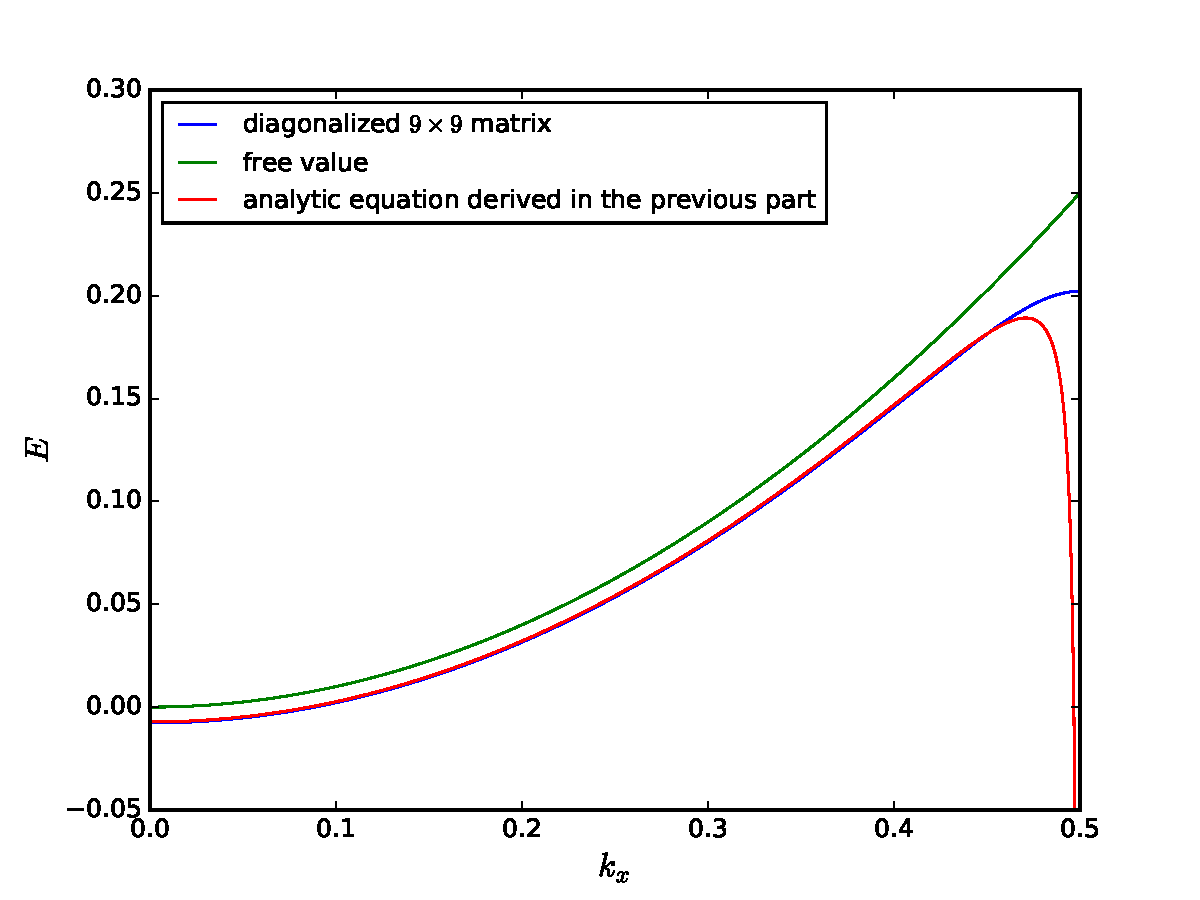
\includegraphics[width=0.7\linewidth]{pro_1_3.pdf}
	      	\caption{$3$ values along path $(0, 0) \rightarrow (\frac{1}{2}, 0)$.}
	      	\label{fig:pro13}
	      \end{figure}
	\item If we want to eliminate the degeneracy for the lowest $2$ bands, we need to reorganize the basis $\Ket{\psi_1^{(0)}}= \exp(i \bm{k}
	      \cdot \bm{r})$ and $\Ket{\psi_3^{(0)}} = \exp(i (\bm{k} + \bm{G}_3) \cdot \bm{r} )$.
	      Suppose the new basis have the form
	      \begin{equation}
	      	\Ket{\phi_\nu^{(0)}} = \sum_\nu c_\nu \exp((\bm{k} + \bm{G}_\nu) \cdot \bm{r}), \quad \nu = 1, 3,
	      \end{equation}
	      with $\Braket{\psi_\mu^{(0)}  | \psi_\nu^{(0)}} = \delta_{\mu\nu}$.
	      Substitute into equation
	      \begin{equation}
	      	\hat{H} \Ket{\phi_\nu^{(0)}} = E_{\nu}^{\text{e}} \Ket{\phi_\nu^{(0)}},
	      \end{equation}
	      here $E_{\nu}^{\text{e}}$ stands for the energy when degeneracy is eliminated.
	      Expand and left multiplied by $\Bra{\phi_\mu^{(0)}}$, where $\mu= 1, 3$, we have
	      \begin{equation}
	      	\sum_{\nu}  c_\nu \Big(  \Braket{\psi_\mu^{(0)} | \hat{H} | \psi_\nu^{(0)} } - E_\nu^{\text{e}} \Braket{\psi_\mu^{(0)}  | \psi_\nu^{(0)}} \Big) = 0,
	      \end{equation}
	      or
	      \begin{equation}
	      	\sum_{\nu}  c_\nu \Big(  \Braket{\psi_\mu^{(0)} | \hat{H} | \psi_\nu^{(0)} } - E_\nu^{\text{e}} \delta_{\mu\nu} \Big) = 0.
	      \end{equation}
	      Here we suppose $H_{\mu\nu} = \Braket{\psi_\mu^{(0)} | \hat{H} | \psi_\nu^{(0)}}$, so
	      \begin{align}
	      	H_{11} & = \Braket{\psi_1^{(0)} | \hat{H}_0 | \psi_1^{(0)}} + \Braket{\psi_1^{(0)} | \hat{H}_1 | \psi_1^{(0)} } = \frac{\hbar^2}{2m} \frac{4\pi^2}{a^2} \Big(k_x^2 + k_y^2 + 0 \Big),     \\
	      	H_{13} & = \Braket{\psi_1^{(0)} | \hat{H}_0 | \psi_3^{(0)}} + \Braket{\psi_1^{(0)} | \hat{H}_1 | \psi_3^{(0)} } = \frac{\hbar^2}{2m} \frac{4\pi^2}{a^2} (0 - 0.04 ),                      \\
	      	H_{31} & = \Braket{\psi_3^{(0)} | \hat{H}_0 | \psi_1^{(0)}} + \Braket{\psi_3^{(0)} | \hat{H}_1 | \psi_1^{(0)} } = \frac{\hbar^2}{2m} \frac{4\pi^2}{a^2} (0 - 0.04 ),                      \\
	      	H_{33} & = \Braket{\psi_3^{(0)} | \hat{H}_0 | \psi_3^{(0)}} + \Braket{\psi_3^{(0)} | \hat{H}_1 | \psi_3^{(0)} } = \frac{\hbar^2}{2m} \frac{4\pi^2}{a^2} \Big((k_x-1)^2 + k_y^2 + 0 \Big).
	      \end{align}
	      Write as matrix form,
	      \begin{equation}
	      	\begin{pmatrix}
	      		H_{11} - E_{\nu}^{\text{e}} & H_{13}                      \\
	      		H_{31}                      & H_{33} - E_{\nu}^{\text{e}} \\
	      	\end{pmatrix}
	      	\colvec{2}{c_1}{c_3} = \colvec{2}{0}{0}.
	      \end{equation}
	      Along the path, we have $k_y=0$. Solve it, we derive eigenvalues
	      \begin{align}
	      	E_{1}^{\text{e}} & = \frac{\hbar^2}{2m} \frac{4\pi^2}{a^2}\frac{1}{2} \Big(2 k_x^2-\sqrt{4 k_x^2-4 k_x+1.0064}-2 k_x+1\Big), \\
	      	E_{3}^{\text{e}} & = \frac{\hbar^2}{2m} \frac{4\pi^2}{a^2}\frac{1}{2} \Big(2 k_x^2+\sqrt{4 k_x^2-4 k_x+1.0064}-2 k_x+1\Big),
	      \end{align}
	      where $E_1$ corresponds to lowest branch, $E_3$ corresponds to second lowest branch.
	      The
	      corresponding eigenvectors are
	      \begin{align}
	      	\begin{pmatrix}
	      	c_1                                                                                                          & c_3                                                                \\
	      	\end{pmatrix}\tran
	      	                                                                                                             & =
	      	\begin{pmatrix}
	      	\frac{12.5 (\sqrt{4 k_x^2-4 k_x+1.0064}-2 k_x+1)}{\sqrt{156.25 (\sqrt{4 k_x^2-4 k_x+1.0064}-2 k_x+1)^2+1}}   & \frac{1}{\sqrt{156.25 (\sqrt{4 k_x^2-4 k_x+1.0064}-2 k_x+1)^2+1}}  \\
	      	\end{pmatrix}\tran, \\
	      	\begin{pmatrix}
	      	c_1'                                                                                                         & c_3'                                                               \\
	      	\end{pmatrix}\tran
	      	                                                                                                             & =
	      	\begin{pmatrix}
	      	\frac{12.5 (-\sqrt{4 k_x^2-4 k_x+1.0064}-2 k_x+1)}{\sqrt{156.25 (-\sqrt{4 k_x^2-4 k_x+1.0064}-2 k_x+1)^2+1}} & \frac{1}{\sqrt{156.25 (-\sqrt{4 k_x^2-4 k_x+1.0064}-2 k_x+1)^2+1}} \\
	      	\end{pmatrix}\tran.
	      \end{align}

	      So new basis are
	      \begin{align}
	      	\Ket{\phi_1^{(0)}} & = c_1 \Ket{\psi_1^{(0)}} + c_3 \Ket{\psi_3^{(0)}} = c_1 \exp((\bm{k} + \bm{G}_1) \cdot \bm{r})
	      	+  c_3 \exp((\bm{k} + \bm{G}_3) \cdot \bm{r}), \\
	      	\Ket{\phi_3^{(0)}} & = c_1' \Ket{\psi_1^{(0)}} + c_3' \Ket{\psi_3^{(0)}} =  c_1' \exp((\bm{k} + \bm{G}_1) \cdot \bm{r})
	      	+  c_3' \exp((\bm{k} + \bm{G}_3) \cdot \bm{r}). \\
	      \end{align}
	      Under these basis, the $2\times 2$ Hamiltonian is diagonalized:
	      \begin{equation}
	      	\begin{pmatrix}
	      		H_{11} & H_{13} \\
	      		H_{31} & H_{33} \\
	      	\end{pmatrix}
	      	\rightarrow
	      	\begin{pmatrix}
	      		E_{1}^{\text{e}} & 0                \\
	      		0                & E_{3}^{\text{e}} \\
	      	\end{pmatrix},
	      \end{equation}
	      where $\nu = 1$, $3$. From here we can see $\bigg\lvert \Braket{\phi_1^{(0)} | \hat{H}_1 | \phi_3^{(0)}} \bigg\rvert^2 = 0$ and $\bigg\lvert \Braket{\phi_3^{(0)} | \hat{H}_1 | \phi_1^{(0)}} \bigg\rvert^2 = 0$.
	      Based on perturbation theory, we know that
	      here
	      \begin{align}
	      	E_1^{\text{e}} & = E_1^{(0)} + E_1^{(1)}, \\
	      	E_3^{\text{e}} & = E_3^{(0)} + E_3^{(1)}.
	      \end{align}
	      So the nest correction is second order correction.

	      Now consider the second order energy corrections,
	      we have
	      \begin{equation}
	      	\begin{split}
	      		E_1^{(2)} &= \sum_{\substack{j\\j\neq 1, 3}} \frac{\Big\lvert \Braket{\psi_j^{(0)} | \hat{H}_1 | \phi_1^{(0)}} \Big\rvert^2}{ \Braket{\phi_1^{(0)} | \hat{H} | \phi_1^{(0)}}
	      			- \Braket{\psi_j^{(0)} | \hat{H}_0 | \psi_j^{(0)}}} \\
	      		&=  \sum_{\substack{j\\j\neq 1, 3}} \frac{\Big\lvert c_1 \Braket{\psi_j^{(0)} | \hat{H}_1 | \psi_1^{(0)}} + c_3 \Braket{\psi_j^{(0)} | \hat{H}_1 | \psi_3^{(0)}} \Big\rvert^2}{ E_1^{\text{e}}
	      			- \Braket{\psi_j^{(0)} | \hat{H}_0 | \psi_j^{(0)}}},
	      	\end{split}
	      \end{equation}
	      and
	      \begin{equation}
	      	\begin{split}
	      		E_3^{(2)} &= \sum_{\substack{j\\j\neq 1, 3}} \frac{\Big\lvert \Braket{\psi_j^{(0)} | \hat{H}_1 | \phi_3^{(0)}} \Big\rvert^2}{ \Braket{\phi_3^{(0)} | \hat{H} | \phi_3^{(0)}}
	      			- \Braket{\psi_j^{(0)} | \hat{H}_0 | \psi_j^{(0)}}} \\
	      		&=  \sum_{\substack{j\\j\neq 1, 3}} \frac{\Big\lvert c_1' \Braket{\psi_j^{(0)} | \hat{H}_1 | \psi_1^{(0)}} + c_3' \Braket{\psi_j^{(0)} | \hat{H}_1 | \psi_3^{(0)}} \Big\rvert^2}{ E_3^{\text{e}}
	      			- \Braket{\psi_j^{(0)} | \hat{H}_0 | \psi_j^{(0)}}},
	      	\end{split}
	      \end{equation}
	      the expansion of these functions are too complicated, and I will not write it here.
	      Add these values to the original eigenvalues, we have total energy
	      \begin{align}
	      	E_1 = E_{1}^{\text{e}} + E_1^{(2)} & = \frac{\hbar^2\pi^2}{ma^2} \Big(2 k_x^2-\sqrt{4 k_x^2-4 k_x+1.0064}-2 k_x+1\Big) + \sum_{\substack{j  \\j\neq 1, 3}} \frac{\Big\lvert \Braket{\psi_j^{(0)} | \hat{H}_1 | \phi_1^{(0)}} \Big\rvert^2}{ \Braket{\phi_1^{(0)} | \hat{H} | \phi_1^{(0)}}
	      	- \Braket{\psi_j^{(0)} | \hat{H}_0 | \psi_j^{(0)}}}, \\
	      	E_3 = E_{3}^{\text{e}} + E_3^{(2)} & =  \frac{\hbar^2\pi^2}{ma^2} \Big(2 k_x^2+\sqrt{4 k_x^2-4 k_x+1.0064}-2 k_x+1\Big) + \sum_{\substack{j \\j\neq 1, 3}} \frac{\Big\lvert \Braket{\psi_j^{(0)} | \hat{H}_1 | \phi_3^{(0)}} \Big\rvert^2}{ \Braket{\phi_3^{(0)} | \hat{H} | \phi_3^{(0)}}
	      	- \Braket{\psi_j^{(0)} | \hat{H}_0 | \psi_j^{(0)}}}.
	      \end{align}
	      Here $E_1$ is the energy of the lowest branch, is what we will plot.
	      See Fig. \ref{fig:pro14} for results, where $k_x$ is dimensionless, and $E$ is of unit $\frac{\hbar^2}{2m}\frac{4\pi^2}{a^2}$.
	      From this figure, we can see second order correction is already a good approximation, which overlaps with $9\times 9$ matrix curve.
	      \begin{figure}[h]
	      	\centering
	      	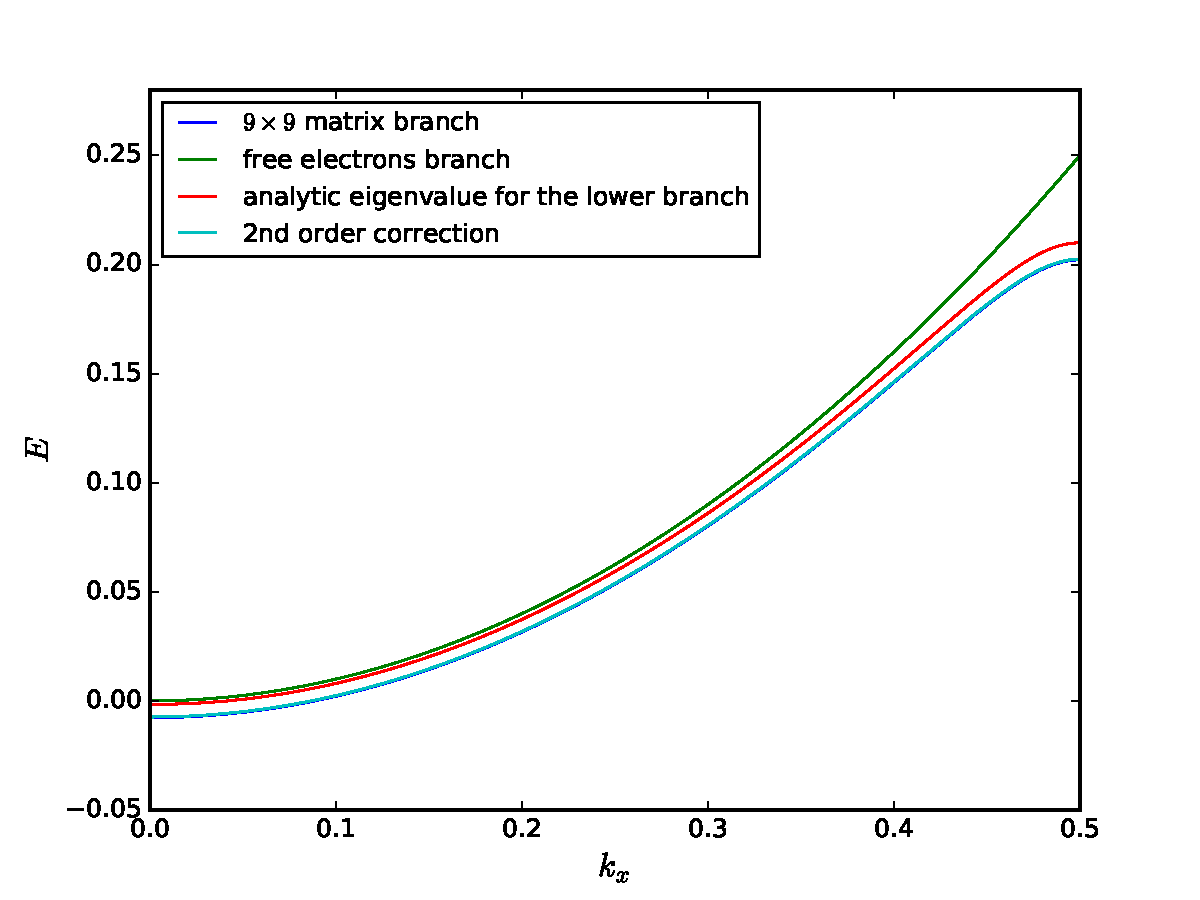
\includegraphics[width=0.7\linewidth]{pro_1_4.pdf}
	      	\caption{4 values along path $(0, 0) \rightarrow (\frac{1}{2}, 0)$.}
	      	\label{fig:pro14}
	      \end{figure}

\end{enumerate}


\section*{Problem \RMN{2}}
\begin{enumerate}[(a)]
	\item
	      \begin{figure}[h]
	      	\centering
	      	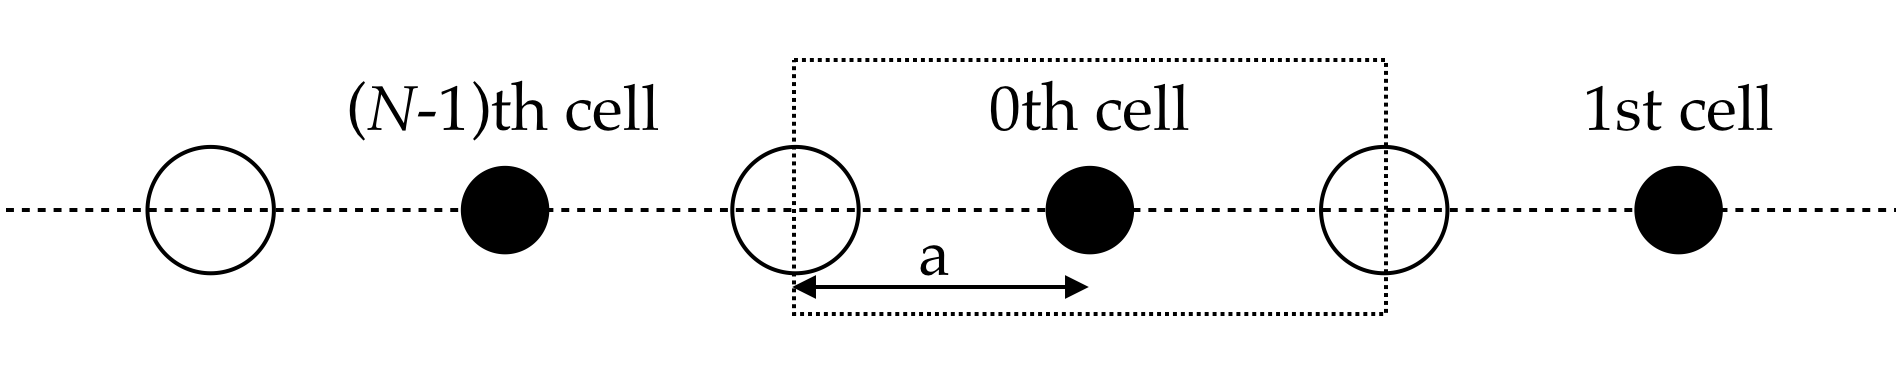
\includegraphics[width=0.7\linewidth]{question 2.png}
	      	\caption{One dimensional lattice with some potential.}
	      	\label{fig:question-2}
	      \end{figure}

	      Consider a unit cell to be of $2a$ length, where $a$ is the length between $2$ Hydrogen s-orbital. See Fig. \ref{fig:question-2} for reference.
	      We use the eigenvectors of translation group to block diagonal Hamiltonian, here the eigenvectors have form
	      \begin{equation}
	      	\psi_{\bm{k}} = \frac{1}{\sqrt{N}} \sum_{\nu} \sum_{\bm{R}}  \exp(i \bm{k} \cdot \bm{R}) \phi_\nu(\bm{r} - \bm{R}).
	      \end{equation}
	      So
	      \begin{equation}\label{eq:hamiltonian}
	      	\begin{split}
	      		H(\bm{k})
	      		&= \braket{\psi_{\bm{k}'}^\ast(\bm{r})| \hat{H} |\psi_{\bm{k}}(\bm{r})}\\
	      		&= \frac{1}{N}\sum_{\bm{R}\bm{R}'}\sum_{\mu,\nu} \exp(i(\bm{k}-\bm{k}')\cdot \bm{R}') \exp(i\bm{k}\cdot\bm{R}) \braket{\phi_\mu(\bm{r}) | \hat{H} | \phi_\nu(\bm{r} - \bm{R})}\\
	      		&= \sum_{\bm{R}}\sum_{\mu,\nu} \delta_{\bm{k}'\bm{k}}\exp(i\bm{k}\cdot \bm{R}) \braket{\phi_\mu(\bm{r}) | \hat{H} | \phi_\nu(\bm{r} - \bm{R})}
	      	\end{split}
	      \end{equation}
	      where $\phi(\bm{r} - \bm{R})$ is the s-orbital located at a lattice vector $\bm{R}$ from origin, $\bm{k}$ and $\bm{k}'$ are wave vectors, $\mu$ and $\nu$ means considering different types of orbitals.
	      Now consider the $0$th cell, it has two basis, the ``white'' s-orbital $\phi_\alpha(\bm{r})$ and the ``black'' orbital $\phi_\beta(\bm{r})$,
	      with relations
	      \begin{align}
	      	\braket{\phi_\alpha(\bm{r}) | \hat{H} | \phi_\alpha(\bm{r})} & = \varepsilon_0 + \varepsilon, \\
	      	\braket{\phi_\alpha(\bm{r}) | \hat{H} | \phi_\beta(\bm{r})}  & = t,                           \\
	      	\braket{\phi_\beta(\bm{r}) | \hat{H} | \phi_\alpha(\bm{r})}  & = t,                           \\
	      	\braket{\phi_\beta(\bm{r}) | \hat{H} | \phi_\beta(\bm{r})}   & = \varepsilon_0 - \varepsilon,
	      \end{align}
	      so the Hamiltonian matrix under these two basis will be
	      \begin{equation}
	      	H(\bm{R} = \bm{0}) =
	      	\begin{pmatrix}
	      		\varepsilon_0 + \varepsilon & t                           \\
	      		t                           & \varepsilon_0 - \varepsilon \\
	      	\end{pmatrix},
	      \end{equation}
	      where $t$ is the nearest neighbor hopping term. Now let's consider the $1$st unit cell, here $\bm{R} = 2\bm{a}$.
	      As above, we write down its relations
	      \begin{align}
	      	\braket{\phi_\alpha(\bm{r}) | \hat{H} | \phi_\alpha(\bm{r} - 2\bm{a})} = 0, \\
	      	\braket{\phi_\alpha(\bm{r}) | \hat{H} | \phi_\beta(\bm{r} - 2\bm{a})} = 0,  \\
	      	\braket{\phi_\beta(\bm{r}) | \hat{H} | \phi_\alpha(\bm{r} - 2\bm{a})} = t,  \\
	      	\braket{\phi_\beta(\bm{r}) | \hat{H} | \phi_\beta(\bm{r} - 2\bm{a})} = 0,
	      \end{align}
	      so again, the Hamiltonian matrix under these two basis will be
	      \begin{equation}
	      	H(\bm{R} = 2\bm{a}) =
	      	\begin{pmatrix}
	      		0 & 0 \\
	      		t & 0 \\
	      	\end{pmatrix}.
	      \end{equation}
	      At last, the $(N-1)$th unit cell, with $\bm{R} = (N-1) 2\bm{a} \equiv - 2\bm{a}$, has relations
	      \begin{align}
	      	\braket{\phi_\alpha(\bm{r}) | \hat{H} | \phi_\alpha(\bm{r} + 2\bm{a})} = 0, \\
	      	\braket{\phi_\alpha(\bm{r}) | \hat{H} | \phi_\beta(\bm{r} + 2\bm{a})} = t,  \\
	      	\braket{\phi_\beta(\bm{r}) | \hat{H} | \phi_\alpha(\bm{r} + 2\bm{a})} = 0,  \\
	      	\braket{\phi_\beta(\bm{r}) | \hat{H} | \phi_\beta(\bm{r} + 2\bm{a})} = 0.
	      \end{align}
	      So the last Hamiltonian matrix under the basis is
	      \begin{equation}
	      	H(\bm{R} = -2\bm{a}) =
	      	\begin{pmatrix}
	      		0 & t \\
	      		0 & 0 \\
	      	\end{pmatrix}.
	      \end{equation}
	      Use \eqref{eq:hamiltonian}, we derive total Hamiltonian of the system
	      \begin{equation}
	      	\begin{split}
	      		H(\bm{k}) &=  \sum_{\bm{R}}\sum_{\mu,\nu} \exp(i\bm{k}\cdot \bm{R}) \braket{\phi_\mu(\bm{r}) | \hat{H} | \phi_\nu(\bm{r} - \bm{R})} \\
	      		&=
	      		\begin{pmatrix}
	      			\varepsilon_0 + \varepsilon & t                           \\
	      			t                           & \varepsilon_0 - \varepsilon \\
	      		\end{pmatrix} + \exp(2ika)
	      		\begin{pmatrix}
	      			0 & 0 \\
	      			t & 0 \\
	      		\end{pmatrix} +
	      		\exp(-2ika)
	      		\begin{pmatrix}
	      			0 & t \\
	      			0 & 0 \\
	      		\end{pmatrix},
	      	\end{split}
	      \end{equation}
	      where $\mu$ and $\nu$ denotes different orbitals.
	      Diagonalize this matrix and plot eigenvalues, will be as Fig. \ref{fig:pro2}. Note that there is a very small band gap in $k = \frac{\pi}{2a}$.
	      \begin{figure}[h]
	      	\centering
	      	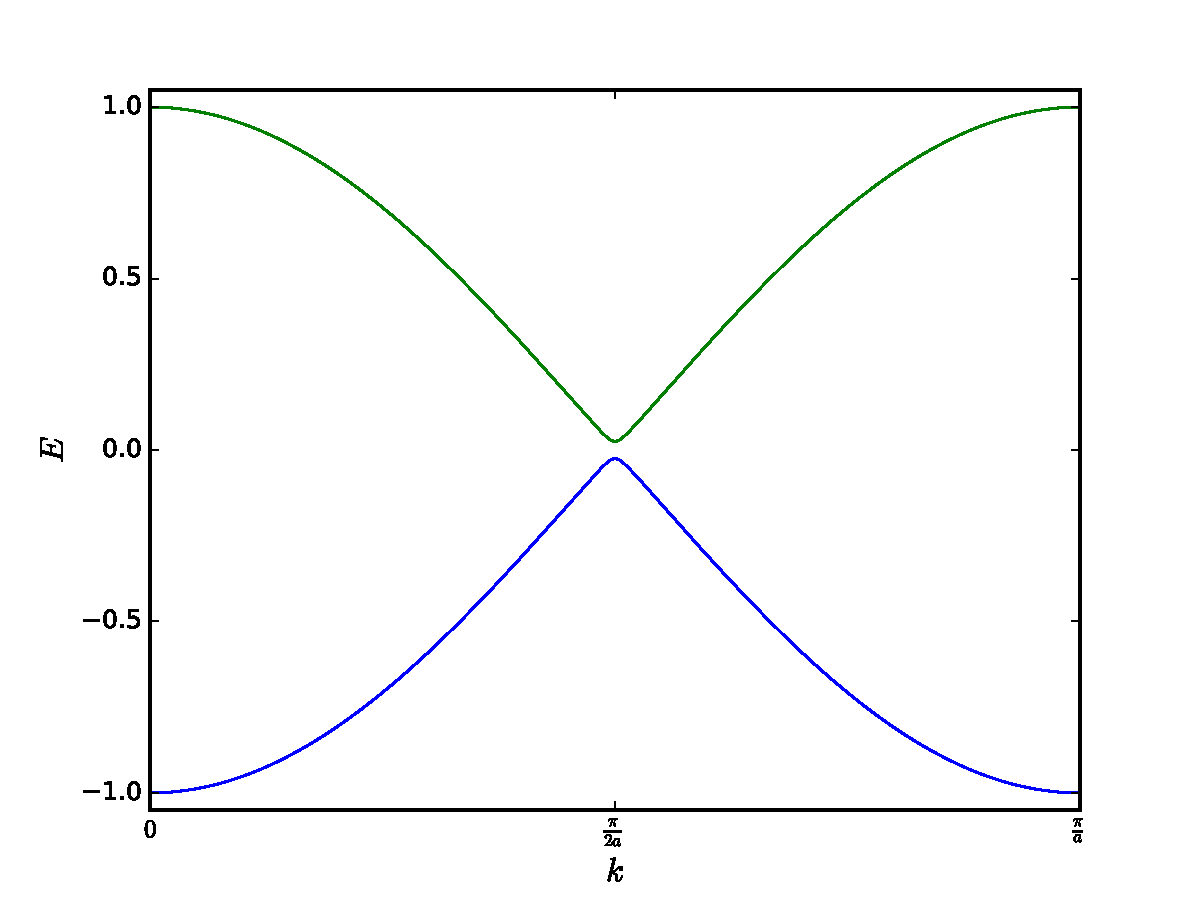
\includegraphics[width=0.7\linewidth]{pro_2.pdf}
	      	\caption{Analytic solution for the band structure.}
	      	\label{fig:pro2}
	      \end{figure}
	\item Suppose there are $N$ unit cells in the lattice, because there is one electron per site, so there are $2N$ electrons in the lattice. Because in first Brillouin zone, there are $N$ k-points, each k-point can hold $2$ electrons, so one band can hold $2N$ electrons in the first Brillouin zone, so the electrons fill up the lower band of the first Brillouin zone. Since the length of the unit cell is $2a$, the the first Brillouin zone boundary locates at $\frac{\pi}{2a}$, as we already saw, there is a small gap. So, it cannot be a metal, it is an insulator.
\end{enumerate}
\end{document}
